% Sampled Games: Learned Listener
%
% Build:  tectonic docs/sampled-games-learned-listener.tex
% Output: docs/sampled-games-learned-listener.pdf
%
% Companion to clue-selection-theory.tex's worked game, same rendering, for
% the learned_listener spymaster. Generated by
%   python scripts/tools/render_game_tikz.py --seed S --side X \
%       --model learned_listener --label-like 'learned_listener%'
% Three games drawn at random from those it won by revealing all of its own
% words. Gold outlines are the words the clue was meant for, recovered by
% rescoring the clue with the distilled listener over the unrevealed board.

\documentclass[12pt]{article}

\usepackage[a4paper,margin=3.2cm]{geometry}
\usepackage{amsmath}
\usepackage{caption}
\usepackage{float}
\usepackage[skip=8pt, indent=0pt]{parskip}
\usepackage{microtype}
\usepackage[T1]{fontenc}
\usepackage{libertinus}
\usepackage{xcolor}
\usepackage{tikz}

\definecolor{cnblue}{HTML}{3A6EA5}
\definecolor{cnred}{HTML}{B4504D}
\definecolor{cntan}{HTML}{D9CBA3}
\definecolor{cnblack}{HTML}{2B2B2B}
\definecolor{cngold}{HTML}{C99A2E}

\pagestyle{empty}

\begin{document}

\begin{center}
  {\LARGE Sampled Games}\\[0.7em]
  Codenames spymaster, learned listener
\end{center}
\vspace{1.5em}

\section*{Game 1}

\begin{figure}[H]
\centering
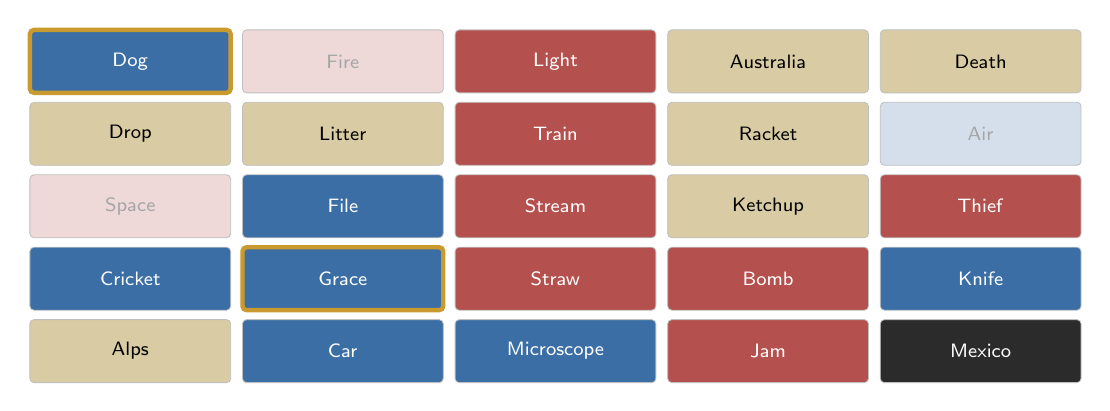
\begin{tikzpicture}[x=2.7cm, y=0.92cm]
  \node[draw=cngold, line width=1.6pt, fill=cnblue, minimum width=2.55cm, minimum height=0.8cm, inner sep=1pt, rounded corners=1.5pt] at (0,0) {\textcolor{white}{\scriptsize\textsf{Dog}}};
  \node[draw=black!25, line width=0.3pt, fill=cnred!22, minimum width=2.55cm, minimum height=0.8cm, inner sep=1pt, rounded corners=1.5pt] at (1,0) {\textcolor{black!35}{\scriptsize\textsf{Fire}}};
  \node[draw=black!25, line width=0.3pt, fill=cnred, minimum width=2.55cm, minimum height=0.8cm, inner sep=1pt, rounded corners=1.5pt] at (2,0) {\textcolor{white}{\scriptsize\textsf{Light}}};
  \node[draw=black!25, line width=0.3pt, fill=cntan, minimum width=2.55cm, minimum height=0.8cm, inner sep=1pt, rounded corners=1.5pt] at (3,0) {\textcolor{black}{\scriptsize\textsf{Australia}}};
  \node[draw=black!25, line width=0.3pt, fill=cntan, minimum width=2.55cm, minimum height=0.8cm, inner sep=1pt, rounded corners=1.5pt] at (4,0) {\textcolor{black}{\scriptsize\textsf{Death}}};
  \node[draw=black!25, line width=0.3pt, fill=cntan, minimum width=2.55cm, minimum height=0.8cm, inner sep=1pt, rounded corners=1.5pt] at (0,-1) {\textcolor{black}{\scriptsize\textsf{Drop}}};
  \node[draw=black!25, line width=0.3pt, fill=cntan, minimum width=2.55cm, minimum height=0.8cm, inner sep=1pt, rounded corners=1.5pt] at (1,-1) {\textcolor{black}{\scriptsize\textsf{Litter}}};
  \node[draw=black!25, line width=0.3pt, fill=cnred, minimum width=2.55cm, minimum height=0.8cm, inner sep=1pt, rounded corners=1.5pt] at (2,-1) {\textcolor{white}{\scriptsize\textsf{Train}}};
  \node[draw=black!25, line width=0.3pt, fill=cntan, minimum width=2.55cm, minimum height=0.8cm, inner sep=1pt, rounded corners=1.5pt] at (3,-1) {\textcolor{black}{\scriptsize\textsf{Racket}}};
  \node[draw=black!25, line width=0.3pt, fill=cnblue!22, minimum width=2.55cm, minimum height=0.8cm, inner sep=1pt, rounded corners=1.5pt] at (4,-1) {\textcolor{black!35}{\scriptsize\textsf{Air}}};
  \node[draw=black!25, line width=0.3pt, fill=cnred!22, minimum width=2.55cm, minimum height=0.8cm, inner sep=1pt, rounded corners=1.5pt] at (0,-2) {\textcolor{black!35}{\scriptsize\textsf{Space}}};
  \node[draw=black!25, line width=0.3pt, fill=cnblue, minimum width=2.55cm, minimum height=0.8cm, inner sep=1pt, rounded corners=1.5pt] at (1,-2) {\textcolor{white}{\scriptsize\textsf{File}}};
  \node[draw=black!25, line width=0.3pt, fill=cnred, minimum width=2.55cm, minimum height=0.8cm, inner sep=1pt, rounded corners=1.5pt] at (2,-2) {\textcolor{white}{\scriptsize\textsf{Stream}}};
  \node[draw=black!25, line width=0.3pt, fill=cntan, minimum width=2.55cm, minimum height=0.8cm, inner sep=1pt, rounded corners=1.5pt] at (3,-2) {\textcolor{black}{\scriptsize\textsf{Ketchup}}};
  \node[draw=black!25, line width=0.3pt, fill=cnred, minimum width=2.55cm, minimum height=0.8cm, inner sep=1pt, rounded corners=1.5pt] at (4,-2) {\textcolor{white}{\scriptsize\textsf{Thief}}};
  \node[draw=black!25, line width=0.3pt, fill=cnblue, minimum width=2.55cm, minimum height=0.8cm, inner sep=1pt, rounded corners=1.5pt] at (0,-3) {\textcolor{white}{\scriptsize\textsf{Cricket}}};
  \node[draw=cngold, line width=1.6pt, fill=cnblue, minimum width=2.55cm, minimum height=0.8cm, inner sep=1pt, rounded corners=1.5pt] at (1,-3) {\textcolor{white}{\scriptsize\textsf{Grace}}};
  \node[draw=black!25, line width=0.3pt, fill=cnred, minimum width=2.55cm, minimum height=0.8cm, inner sep=1pt, rounded corners=1.5pt] at (2,-3) {\textcolor{white}{\scriptsize\textsf{Straw}}};
  \node[draw=black!25, line width=0.3pt, fill=cnred, minimum width=2.55cm, minimum height=0.8cm, inner sep=1pt, rounded corners=1.5pt] at (3,-3) {\textcolor{white}{\scriptsize\textsf{Bomb}}};
  \node[draw=black!25, line width=0.3pt, fill=cnblue, minimum width=2.55cm, minimum height=0.8cm, inner sep=1pt, rounded corners=1.5pt] at (4,-3) {\textcolor{white}{\scriptsize\textsf{Knife}}};
  \node[draw=black!25, line width=0.3pt, fill=cntan, minimum width=2.55cm, minimum height=0.8cm, inner sep=1pt, rounded corners=1.5pt] at (0,-4) {\textcolor{black}{\scriptsize\textsf{Alps}}};
  \node[draw=black!25, line width=0.3pt, fill=cnblue, minimum width=2.55cm, minimum height=0.8cm, inner sep=1pt, rounded corners=1.5pt] at (1,-4) {\textcolor{white}{\scriptsize\textsf{Car}}};
  \node[draw=black!25, line width=0.3pt, fill=cnblue, minimum width=2.55cm, minimum height=0.8cm, inner sep=1pt, rounded corners=1.5pt] at (2,-4) {\textcolor{white}{\scriptsize\textsf{Microscope}}};
  \node[draw=black!25, line width=0.3pt, fill=cnred, minimum width=2.55cm, minimum height=0.8cm, inner sep=1pt, rounded corners=1.5pt] at (3,-4) {\textcolor{white}{\scriptsize\textsf{Jam}}};
  \node[draw=black!25, line width=0.3pt, fill=cnblack, minimum width=2.55cm, minimum height=0.8cm, inner sep=1pt, rounded corners=1.5pt] at (4,-4) {\textcolor{white}{\scriptsize\textsf{Mexico}}};
\end{tikzpicture}
\caption*{\footnotesize \textbf{Turn 1} --- clue \textsc{affection} 2. Guesser took: \textbf{Dog}, \textbf{Grace}.}
\end{figure}

\begin{figure}[H]
\centering
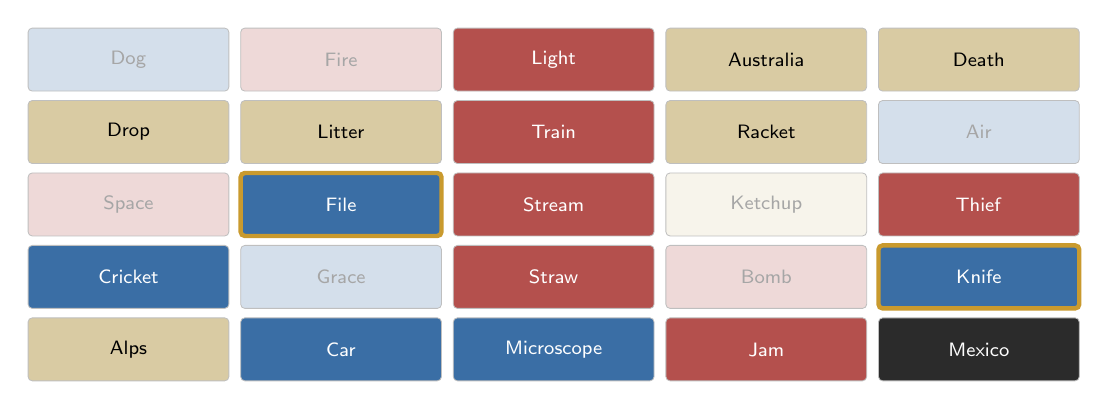
\begin{tikzpicture}[x=2.7cm, y=0.92cm]
  \node[draw=black!25, line width=0.3pt, fill=cnblue!22, minimum width=2.55cm, minimum height=0.8cm, inner sep=1pt, rounded corners=1.5pt] at (0,0) {\textcolor{black!35}{\scriptsize\textsf{Dog}}};
  \node[draw=black!25, line width=0.3pt, fill=cnred!22, minimum width=2.55cm, minimum height=0.8cm, inner sep=1pt, rounded corners=1.5pt] at (1,0) {\textcolor{black!35}{\scriptsize\textsf{Fire}}};
  \node[draw=black!25, line width=0.3pt, fill=cnred, minimum width=2.55cm, minimum height=0.8cm, inner sep=1pt, rounded corners=1.5pt] at (2,0) {\textcolor{white}{\scriptsize\textsf{Light}}};
  \node[draw=black!25, line width=0.3pt, fill=cntan, minimum width=2.55cm, minimum height=0.8cm, inner sep=1pt, rounded corners=1.5pt] at (3,0) {\textcolor{black}{\scriptsize\textsf{Australia}}};
  \node[draw=black!25, line width=0.3pt, fill=cntan, minimum width=2.55cm, minimum height=0.8cm, inner sep=1pt, rounded corners=1.5pt] at (4,0) {\textcolor{black}{\scriptsize\textsf{Death}}};
  \node[draw=black!25, line width=0.3pt, fill=cntan, minimum width=2.55cm, minimum height=0.8cm, inner sep=1pt, rounded corners=1.5pt] at (0,-1) {\textcolor{black}{\scriptsize\textsf{Drop}}};
  \node[draw=black!25, line width=0.3pt, fill=cntan, minimum width=2.55cm, minimum height=0.8cm, inner sep=1pt, rounded corners=1.5pt] at (1,-1) {\textcolor{black}{\scriptsize\textsf{Litter}}};
  \node[draw=black!25, line width=0.3pt, fill=cnred, minimum width=2.55cm, minimum height=0.8cm, inner sep=1pt, rounded corners=1.5pt] at (2,-1) {\textcolor{white}{\scriptsize\textsf{Train}}};
  \node[draw=black!25, line width=0.3pt, fill=cntan, minimum width=2.55cm, minimum height=0.8cm, inner sep=1pt, rounded corners=1.5pt] at (3,-1) {\textcolor{black}{\scriptsize\textsf{Racket}}};
  \node[draw=black!25, line width=0.3pt, fill=cnblue!22, minimum width=2.55cm, minimum height=0.8cm, inner sep=1pt, rounded corners=1.5pt] at (4,-1) {\textcolor{black!35}{\scriptsize\textsf{Air}}};
  \node[draw=black!25, line width=0.3pt, fill=cnred!22, minimum width=2.55cm, minimum height=0.8cm, inner sep=1pt, rounded corners=1.5pt] at (0,-2) {\textcolor{black!35}{\scriptsize\textsf{Space}}};
  \node[draw=cngold, line width=1.6pt, fill=cnblue, minimum width=2.55cm, minimum height=0.8cm, inner sep=1pt, rounded corners=1.5pt] at (1,-2) {\textcolor{white}{\scriptsize\textsf{File}}};
  \node[draw=black!25, line width=0.3pt, fill=cnred, minimum width=2.55cm, minimum height=0.8cm, inner sep=1pt, rounded corners=1.5pt] at (2,-2) {\textcolor{white}{\scriptsize\textsf{Stream}}};
  \node[draw=black!25, line width=0.3pt, fill=cntan!22, minimum width=2.55cm, minimum height=0.8cm, inner sep=1pt, rounded corners=1.5pt] at (3,-2) {\textcolor{black!35}{\scriptsize\textsf{Ketchup}}};
  \node[draw=black!25, line width=0.3pt, fill=cnred, minimum width=2.55cm, minimum height=0.8cm, inner sep=1pt, rounded corners=1.5pt] at (4,-2) {\textcolor{white}{\scriptsize\textsf{Thief}}};
  \node[draw=black!25, line width=0.3pt, fill=cnblue, minimum width=2.55cm, minimum height=0.8cm, inner sep=1pt, rounded corners=1.5pt] at (0,-3) {\textcolor{white}{\scriptsize\textsf{Cricket}}};
  \node[draw=black!25, line width=0.3pt, fill=cnblue!22, minimum width=2.55cm, minimum height=0.8cm, inner sep=1pt, rounded corners=1.5pt] at (1,-3) {\textcolor{black!35}{\scriptsize\textsf{Grace}}};
  \node[draw=black!25, line width=0.3pt, fill=cnred, minimum width=2.55cm, minimum height=0.8cm, inner sep=1pt, rounded corners=1.5pt] at (2,-3) {\textcolor{white}{\scriptsize\textsf{Straw}}};
  \node[draw=black!25, line width=0.3pt, fill=cnred!22, minimum width=2.55cm, minimum height=0.8cm, inner sep=1pt, rounded corners=1.5pt] at (3,-3) {\textcolor{black!35}{\scriptsize\textsf{Bomb}}};
  \node[draw=cngold, line width=1.6pt, fill=cnblue, minimum width=2.55cm, minimum height=0.8cm, inner sep=1pt, rounded corners=1.5pt] at (4,-3) {\textcolor{white}{\scriptsize\textsf{Knife}}};
  \node[draw=black!25, line width=0.3pt, fill=cntan, minimum width=2.55cm, minimum height=0.8cm, inner sep=1pt, rounded corners=1.5pt] at (0,-4) {\textcolor{black}{\scriptsize\textsf{Alps}}};
  \node[draw=black!25, line width=0.3pt, fill=cnblue, minimum width=2.55cm, minimum height=0.8cm, inner sep=1pt, rounded corners=1.5pt] at (1,-4) {\textcolor{white}{\scriptsize\textsf{Car}}};
  \node[draw=black!25, line width=0.3pt, fill=cnblue, minimum width=2.55cm, minimum height=0.8cm, inner sep=1pt, rounded corners=1.5pt] at (2,-4) {\textcolor{white}{\scriptsize\textsf{Microscope}}};
  \node[draw=black!25, line width=0.3pt, fill=cnred, minimum width=2.55cm, minimum height=0.8cm, inner sep=1pt, rounded corners=1.5pt] at (3,-4) {\textcolor{white}{\scriptsize\textsf{Jam}}};
  \node[draw=black!25, line width=0.3pt, fill=cnblack, minimum width=2.55cm, minimum height=0.8cm, inner sep=1pt, rounded corners=1.5pt] at (4,-4) {\textcolor{white}{\scriptsize\textsf{Mexico}}};
\end{tikzpicture}
\caption*{\footnotesize \textbf{Turn 2} --- clue \textsc{tool} 2. Guesser took: \textbf{File}, \textbf{Knife}.}
\end{figure}

\begin{figure}[H]
\centering
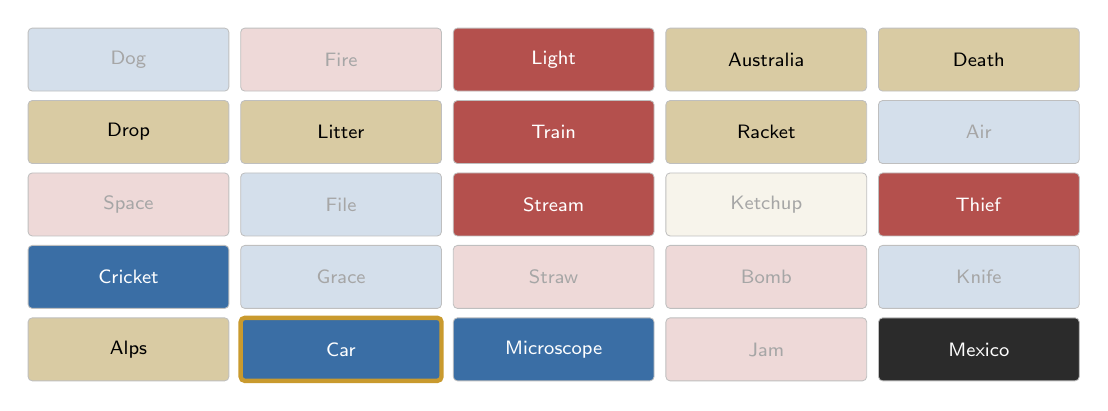
\begin{tikzpicture}[x=2.7cm, y=0.92cm]
  \node[draw=black!25, line width=0.3pt, fill=cnblue!22, minimum width=2.55cm, minimum height=0.8cm, inner sep=1pt, rounded corners=1.5pt] at (0,0) {\textcolor{black!35}{\scriptsize\textsf{Dog}}};
  \node[draw=black!25, line width=0.3pt, fill=cnred!22, minimum width=2.55cm, minimum height=0.8cm, inner sep=1pt, rounded corners=1.5pt] at (1,0) {\textcolor{black!35}{\scriptsize\textsf{Fire}}};
  \node[draw=black!25, line width=0.3pt, fill=cnred, minimum width=2.55cm, minimum height=0.8cm, inner sep=1pt, rounded corners=1.5pt] at (2,0) {\textcolor{white}{\scriptsize\textsf{Light}}};
  \node[draw=black!25, line width=0.3pt, fill=cntan, minimum width=2.55cm, minimum height=0.8cm, inner sep=1pt, rounded corners=1.5pt] at (3,0) {\textcolor{black}{\scriptsize\textsf{Australia}}};
  \node[draw=black!25, line width=0.3pt, fill=cntan, minimum width=2.55cm, minimum height=0.8cm, inner sep=1pt, rounded corners=1.5pt] at (4,0) {\textcolor{black}{\scriptsize\textsf{Death}}};
  \node[draw=black!25, line width=0.3pt, fill=cntan, minimum width=2.55cm, minimum height=0.8cm, inner sep=1pt, rounded corners=1.5pt] at (0,-1) {\textcolor{black}{\scriptsize\textsf{Drop}}};
  \node[draw=black!25, line width=0.3pt, fill=cntan, minimum width=2.55cm, minimum height=0.8cm, inner sep=1pt, rounded corners=1.5pt] at (1,-1) {\textcolor{black}{\scriptsize\textsf{Litter}}};
  \node[draw=black!25, line width=0.3pt, fill=cnred, minimum width=2.55cm, minimum height=0.8cm, inner sep=1pt, rounded corners=1.5pt] at (2,-1) {\textcolor{white}{\scriptsize\textsf{Train}}};
  \node[draw=black!25, line width=0.3pt, fill=cntan, minimum width=2.55cm, minimum height=0.8cm, inner sep=1pt, rounded corners=1.5pt] at (3,-1) {\textcolor{black}{\scriptsize\textsf{Racket}}};
  \node[draw=black!25, line width=0.3pt, fill=cnblue!22, minimum width=2.55cm, minimum height=0.8cm, inner sep=1pt, rounded corners=1.5pt] at (4,-1) {\textcolor{black!35}{\scriptsize\textsf{Air}}};
  \node[draw=black!25, line width=0.3pt, fill=cnred!22, minimum width=2.55cm, minimum height=0.8cm, inner sep=1pt, rounded corners=1.5pt] at (0,-2) {\textcolor{black!35}{\scriptsize\textsf{Space}}};
  \node[draw=black!25, line width=0.3pt, fill=cnblue!22, minimum width=2.55cm, minimum height=0.8cm, inner sep=1pt, rounded corners=1.5pt] at (1,-2) {\textcolor{black!35}{\scriptsize\textsf{File}}};
  \node[draw=black!25, line width=0.3pt, fill=cnred, minimum width=2.55cm, minimum height=0.8cm, inner sep=1pt, rounded corners=1.5pt] at (2,-2) {\textcolor{white}{\scriptsize\textsf{Stream}}};
  \node[draw=black!25, line width=0.3pt, fill=cntan!22, minimum width=2.55cm, minimum height=0.8cm, inner sep=1pt, rounded corners=1.5pt] at (3,-2) {\textcolor{black!35}{\scriptsize\textsf{Ketchup}}};
  \node[draw=black!25, line width=0.3pt, fill=cnred, minimum width=2.55cm, minimum height=0.8cm, inner sep=1pt, rounded corners=1.5pt] at (4,-2) {\textcolor{white}{\scriptsize\textsf{Thief}}};
  \node[draw=black!25, line width=0.3pt, fill=cnblue, minimum width=2.55cm, minimum height=0.8cm, inner sep=1pt, rounded corners=1.5pt] at (0,-3) {\textcolor{white}{\scriptsize\textsf{Cricket}}};
  \node[draw=black!25, line width=0.3pt, fill=cnblue!22, minimum width=2.55cm, minimum height=0.8cm, inner sep=1pt, rounded corners=1.5pt] at (1,-3) {\textcolor{black!35}{\scriptsize\textsf{Grace}}};
  \node[draw=black!25, line width=0.3pt, fill=cnred!22, minimum width=2.55cm, minimum height=0.8cm, inner sep=1pt, rounded corners=1.5pt] at (2,-3) {\textcolor{black!35}{\scriptsize\textsf{Straw}}};
  \node[draw=black!25, line width=0.3pt, fill=cnred!22, minimum width=2.55cm, minimum height=0.8cm, inner sep=1pt, rounded corners=1.5pt] at (3,-3) {\textcolor{black!35}{\scriptsize\textsf{Bomb}}};
  \node[draw=black!25, line width=0.3pt, fill=cnblue!22, minimum width=2.55cm, minimum height=0.8cm, inner sep=1pt, rounded corners=1.5pt] at (4,-3) {\textcolor{black!35}{\scriptsize\textsf{Knife}}};
  \node[draw=black!25, line width=0.3pt, fill=cntan, minimum width=2.55cm, minimum height=0.8cm, inner sep=1pt, rounded corners=1.5pt] at (0,-4) {\textcolor{black}{\scriptsize\textsf{Alps}}};
  \node[draw=cngold, line width=1.6pt, fill=cnblue, minimum width=2.55cm, minimum height=0.8cm, inner sep=1pt, rounded corners=1.5pt] at (1,-4) {\textcolor{white}{\scriptsize\textsf{Car}}};
  \node[draw=black!25, line width=0.3pt, fill=cnblue, minimum width=2.55cm, minimum height=0.8cm, inner sep=1pt, rounded corners=1.5pt] at (2,-4) {\textcolor{white}{\scriptsize\textsf{Microscope}}};
  \node[draw=black!25, line width=0.3pt, fill=cnred!22, minimum width=2.55cm, minimum height=0.8cm, inner sep=1pt, rounded corners=1.5pt] at (3,-4) {\textcolor{black!35}{\scriptsize\textsf{Jam}}};
  \node[draw=black!25, line width=0.3pt, fill=cnblack, minimum width=2.55cm, minimum height=0.8cm, inner sep=1pt, rounded corners=1.5pt] at (4,-4) {\textcolor{white}{\scriptsize\textsf{Mexico}}};
\end{tikzpicture}
\caption*{\footnotesize \textbf{Turn 3} --- clue \textsc{automobile} 1. Guesser took: \textbf{Car}.}
\end{figure}

\begin{figure}[H]
\centering
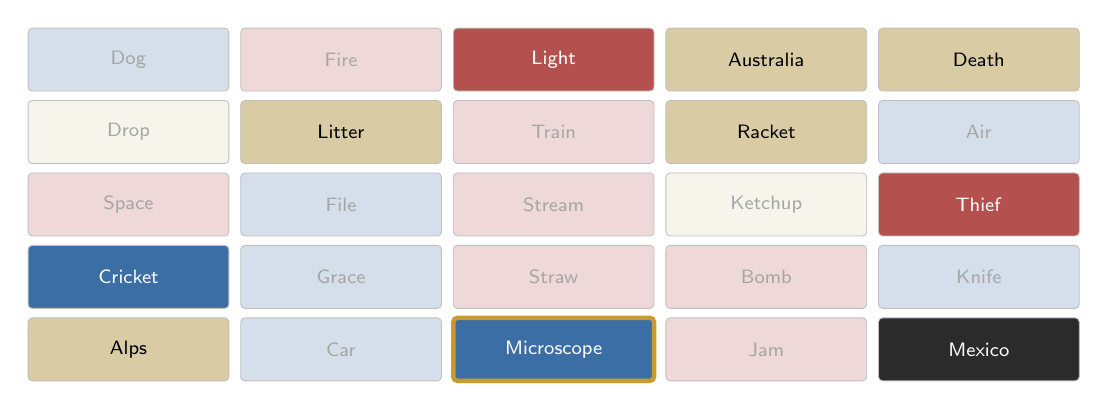
\begin{tikzpicture}[x=2.7cm, y=0.92cm]
  \node[draw=black!25, line width=0.3pt, fill=cnblue!22, minimum width=2.55cm, minimum height=0.8cm, inner sep=1pt, rounded corners=1.5pt] at (0,0) {\textcolor{black!35}{\scriptsize\textsf{Dog}}};
  \node[draw=black!25, line width=0.3pt, fill=cnred!22, minimum width=2.55cm, minimum height=0.8cm, inner sep=1pt, rounded corners=1.5pt] at (1,0) {\textcolor{black!35}{\scriptsize\textsf{Fire}}};
  \node[draw=black!25, line width=0.3pt, fill=cnred, minimum width=2.55cm, minimum height=0.8cm, inner sep=1pt, rounded corners=1.5pt] at (2,0) {\textcolor{white}{\scriptsize\textsf{Light}}};
  \node[draw=black!25, line width=0.3pt, fill=cntan, minimum width=2.55cm, minimum height=0.8cm, inner sep=1pt, rounded corners=1.5pt] at (3,0) {\textcolor{black}{\scriptsize\textsf{Australia}}};
  \node[draw=black!25, line width=0.3pt, fill=cntan, minimum width=2.55cm, minimum height=0.8cm, inner sep=1pt, rounded corners=1.5pt] at (4,0) {\textcolor{black}{\scriptsize\textsf{Death}}};
  \node[draw=black!25, line width=0.3pt, fill=cntan!22, minimum width=2.55cm, minimum height=0.8cm, inner sep=1pt, rounded corners=1.5pt] at (0,-1) {\textcolor{black!35}{\scriptsize\textsf{Drop}}};
  \node[draw=black!25, line width=0.3pt, fill=cntan, minimum width=2.55cm, minimum height=0.8cm, inner sep=1pt, rounded corners=1.5pt] at (1,-1) {\textcolor{black}{\scriptsize\textsf{Litter}}};
  \node[draw=black!25, line width=0.3pt, fill=cnred!22, minimum width=2.55cm, minimum height=0.8cm, inner sep=1pt, rounded corners=1.5pt] at (2,-1) {\textcolor{black!35}{\scriptsize\textsf{Train}}};
  \node[draw=black!25, line width=0.3pt, fill=cntan, minimum width=2.55cm, minimum height=0.8cm, inner sep=1pt, rounded corners=1.5pt] at (3,-1) {\textcolor{black}{\scriptsize\textsf{Racket}}};
  \node[draw=black!25, line width=0.3pt, fill=cnblue!22, minimum width=2.55cm, minimum height=0.8cm, inner sep=1pt, rounded corners=1.5pt] at (4,-1) {\textcolor{black!35}{\scriptsize\textsf{Air}}};
  \node[draw=black!25, line width=0.3pt, fill=cnred!22, minimum width=2.55cm, minimum height=0.8cm, inner sep=1pt, rounded corners=1.5pt] at (0,-2) {\textcolor{black!35}{\scriptsize\textsf{Space}}};
  \node[draw=black!25, line width=0.3pt, fill=cnblue!22, minimum width=2.55cm, minimum height=0.8cm, inner sep=1pt, rounded corners=1.5pt] at (1,-2) {\textcolor{black!35}{\scriptsize\textsf{File}}};
  \node[draw=black!25, line width=0.3pt, fill=cnred!22, minimum width=2.55cm, minimum height=0.8cm, inner sep=1pt, rounded corners=1.5pt] at (2,-2) {\textcolor{black!35}{\scriptsize\textsf{Stream}}};
  \node[draw=black!25, line width=0.3pt, fill=cntan!22, minimum width=2.55cm, minimum height=0.8cm, inner sep=1pt, rounded corners=1.5pt] at (3,-2) {\textcolor{black!35}{\scriptsize\textsf{Ketchup}}};
  \node[draw=black!25, line width=0.3pt, fill=cnred, minimum width=2.55cm, minimum height=0.8cm, inner sep=1pt, rounded corners=1.5pt] at (4,-2) {\textcolor{white}{\scriptsize\textsf{Thief}}};
  \node[draw=black!25, line width=0.3pt, fill=cnblue, minimum width=2.55cm, minimum height=0.8cm, inner sep=1pt, rounded corners=1.5pt] at (0,-3) {\textcolor{white}{\scriptsize\textsf{Cricket}}};
  \node[draw=black!25, line width=0.3pt, fill=cnblue!22, minimum width=2.55cm, minimum height=0.8cm, inner sep=1pt, rounded corners=1.5pt] at (1,-3) {\textcolor{black!35}{\scriptsize\textsf{Grace}}};
  \node[draw=black!25, line width=0.3pt, fill=cnred!22, minimum width=2.55cm, minimum height=0.8cm, inner sep=1pt, rounded corners=1.5pt] at (2,-3) {\textcolor{black!35}{\scriptsize\textsf{Straw}}};
  \node[draw=black!25, line width=0.3pt, fill=cnred!22, minimum width=2.55cm, minimum height=0.8cm, inner sep=1pt, rounded corners=1.5pt] at (3,-3) {\textcolor{black!35}{\scriptsize\textsf{Bomb}}};
  \node[draw=black!25, line width=0.3pt, fill=cnblue!22, minimum width=2.55cm, minimum height=0.8cm, inner sep=1pt, rounded corners=1.5pt] at (4,-3) {\textcolor{black!35}{\scriptsize\textsf{Knife}}};
  \node[draw=black!25, line width=0.3pt, fill=cntan, minimum width=2.55cm, minimum height=0.8cm, inner sep=1pt, rounded corners=1.5pt] at (0,-4) {\textcolor{black}{\scriptsize\textsf{Alps}}};
  \node[draw=black!25, line width=0.3pt, fill=cnblue!22, minimum width=2.55cm, minimum height=0.8cm, inner sep=1pt, rounded corners=1.5pt] at (1,-4) {\textcolor{black!35}{\scriptsize\textsf{Car}}};
  \node[draw=cngold, line width=1.6pt, fill=cnblue, minimum width=2.55cm, minimum height=0.8cm, inner sep=1pt, rounded corners=1.5pt] at (2,-4) {\textcolor{white}{\scriptsize\textsf{Microscope}}};
  \node[draw=black!25, line width=0.3pt, fill=cnred!22, minimum width=2.55cm, minimum height=0.8cm, inner sep=1pt, rounded corners=1.5pt] at (3,-4) {\textcolor{black!35}{\scriptsize\textsf{Jam}}};
  \node[draw=black!25, line width=0.3pt, fill=cnblack, minimum width=2.55cm, minimum height=0.8cm, inner sep=1pt, rounded corners=1.5pt] at (4,-4) {\textcolor{white}{\scriptsize\textsf{Mexico}}};
\end{tikzpicture}
\caption*{\footnotesize \textbf{Turn 4} --- clue \textsc{scrutiny} 1. Guesser took: \textbf{Microscope}.}
\end{figure}


\clearpage

\section*{Game 2}

\begin{figure}[H]
\centering
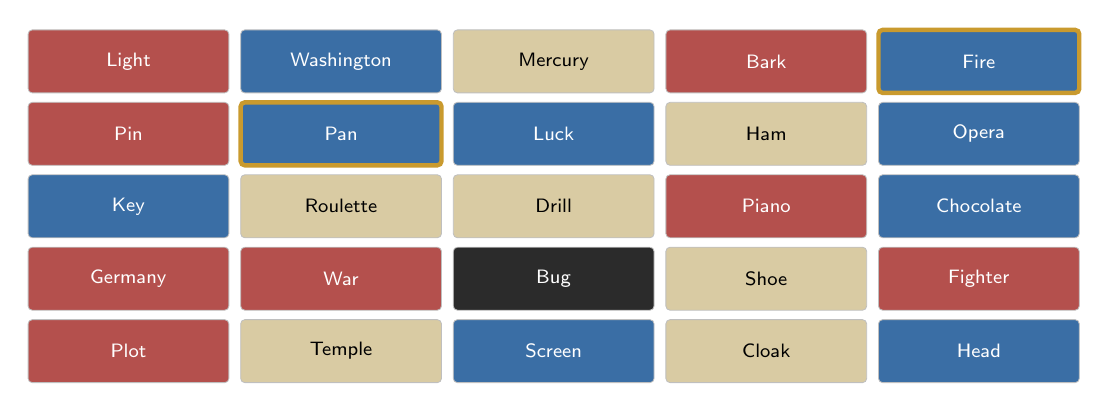
\begin{tikzpicture}[x=2.7cm, y=0.92cm]
  \node[draw=black!25, line width=0.3pt, fill=cnred, minimum width=2.55cm, minimum height=0.8cm, inner sep=1pt, rounded corners=1.5pt] at (0,0) {\textcolor{white}{\scriptsize\textsf{Light}}};
  \node[draw=black!25, line width=0.3pt, fill=cnblue, minimum width=2.55cm, minimum height=0.8cm, inner sep=1pt, rounded corners=1.5pt] at (1,0) {\textcolor{white}{\scriptsize\textsf{Washington}}};
  \node[draw=black!25, line width=0.3pt, fill=cntan, minimum width=2.55cm, minimum height=0.8cm, inner sep=1pt, rounded corners=1.5pt] at (2,0) {\textcolor{black}{\scriptsize\textsf{Mercury}}};
  \node[draw=black!25, line width=0.3pt, fill=cnred, minimum width=2.55cm, minimum height=0.8cm, inner sep=1pt, rounded corners=1.5pt] at (3,0) {\textcolor{white}{\scriptsize\textsf{Bark}}};
  \node[draw=cngold, line width=1.6pt, fill=cnblue, minimum width=2.55cm, minimum height=0.8cm, inner sep=1pt, rounded corners=1.5pt] at (4,0) {\textcolor{white}{\scriptsize\textsf{Fire}}};
  \node[draw=black!25, line width=0.3pt, fill=cnred, minimum width=2.55cm, minimum height=0.8cm, inner sep=1pt, rounded corners=1.5pt] at (0,-1) {\textcolor{white}{\scriptsize\textsf{Pin}}};
  \node[draw=cngold, line width=1.6pt, fill=cnblue, minimum width=2.55cm, minimum height=0.8cm, inner sep=1pt, rounded corners=1.5pt] at (1,-1) {\textcolor{white}{\scriptsize\textsf{Pan}}};
  \node[draw=black!25, line width=0.3pt, fill=cnblue, minimum width=2.55cm, minimum height=0.8cm, inner sep=1pt, rounded corners=1.5pt] at (2,-1) {\textcolor{white}{\scriptsize\textsf{Luck}}};
  \node[draw=black!25, line width=0.3pt, fill=cntan, minimum width=2.55cm, minimum height=0.8cm, inner sep=1pt, rounded corners=1.5pt] at (3,-1) {\textcolor{black}{\scriptsize\textsf{Ham}}};
  \node[draw=black!25, line width=0.3pt, fill=cnblue, minimum width=2.55cm, minimum height=0.8cm, inner sep=1pt, rounded corners=1.5pt] at (4,-1) {\textcolor{white}{\scriptsize\textsf{Opera}}};
  \node[draw=black!25, line width=0.3pt, fill=cnblue, minimum width=2.55cm, minimum height=0.8cm, inner sep=1pt, rounded corners=1.5pt] at (0,-2) {\textcolor{white}{\scriptsize\textsf{Key}}};
  \node[draw=black!25, line width=0.3pt, fill=cntan, minimum width=2.55cm, minimum height=0.8cm, inner sep=1pt, rounded corners=1.5pt] at (1,-2) {\textcolor{black}{\scriptsize\textsf{Roulette}}};
  \node[draw=black!25, line width=0.3pt, fill=cntan, minimum width=2.55cm, minimum height=0.8cm, inner sep=1pt, rounded corners=1.5pt] at (2,-2) {\textcolor{black}{\scriptsize\textsf{Drill}}};
  \node[draw=black!25, line width=0.3pt, fill=cnred, minimum width=2.55cm, minimum height=0.8cm, inner sep=1pt, rounded corners=1.5pt] at (3,-2) {\textcolor{white}{\scriptsize\textsf{Piano}}};
  \node[draw=black!25, line width=0.3pt, fill=cnblue, minimum width=2.55cm, minimum height=0.8cm, inner sep=1pt, rounded corners=1.5pt] at (4,-2) {\textcolor{white}{\scriptsize\textsf{Chocolate}}};
  \node[draw=black!25, line width=0.3pt, fill=cnred, minimum width=2.55cm, minimum height=0.8cm, inner sep=1pt, rounded corners=1.5pt] at (0,-3) {\textcolor{white}{\scriptsize\textsf{Germany}}};
  \node[draw=black!25, line width=0.3pt, fill=cnred, minimum width=2.55cm, minimum height=0.8cm, inner sep=1pt, rounded corners=1.5pt] at (1,-3) {\textcolor{white}{\scriptsize\textsf{War}}};
  \node[draw=black!25, line width=0.3pt, fill=cnblack, minimum width=2.55cm, minimum height=0.8cm, inner sep=1pt, rounded corners=1.5pt] at (2,-3) {\textcolor{white}{\scriptsize\textsf{Bug}}};
  \node[draw=black!25, line width=0.3pt, fill=cntan, minimum width=2.55cm, minimum height=0.8cm, inner sep=1pt, rounded corners=1.5pt] at (3,-3) {\textcolor{black}{\scriptsize\textsf{Shoe}}};
  \node[draw=black!25, line width=0.3pt, fill=cnred, minimum width=2.55cm, minimum height=0.8cm, inner sep=1pt, rounded corners=1.5pt] at (4,-3) {\textcolor{white}{\scriptsize\textsf{Fighter}}};
  \node[draw=black!25, line width=0.3pt, fill=cnred, minimum width=2.55cm, minimum height=0.8cm, inner sep=1pt, rounded corners=1.5pt] at (0,-4) {\textcolor{white}{\scriptsize\textsf{Plot}}};
  \node[draw=black!25, line width=0.3pt, fill=cntan, minimum width=2.55cm, minimum height=0.8cm, inner sep=1pt, rounded corners=1.5pt] at (1,-4) {\textcolor{black}{\scriptsize\textsf{Temple}}};
  \node[draw=black!25, line width=0.3pt, fill=cnblue, minimum width=2.55cm, minimum height=0.8cm, inner sep=1pt, rounded corners=1.5pt] at (2,-4) {\textcolor{white}{\scriptsize\textsf{Screen}}};
  \node[draw=black!25, line width=0.3pt, fill=cntan, minimum width=2.55cm, minimum height=0.8cm, inner sep=1pt, rounded corners=1.5pt] at (3,-4) {\textcolor{black}{\scriptsize\textsf{Cloak}}};
  \node[draw=black!25, line width=0.3pt, fill=cnblue, minimum width=2.55cm, minimum height=0.8cm, inner sep=1pt, rounded corners=1.5pt] at (4,-4) {\textcolor{white}{\scriptsize\textsf{Head}}};
\end{tikzpicture}
\caption*{\footnotesize \textbf{Turn 1} --- clue \textsc{stove} 2. Guesser took: \textbf{Fire}, \textbf{Pan}.}
\end{figure}

\begin{figure}[H]
\centering
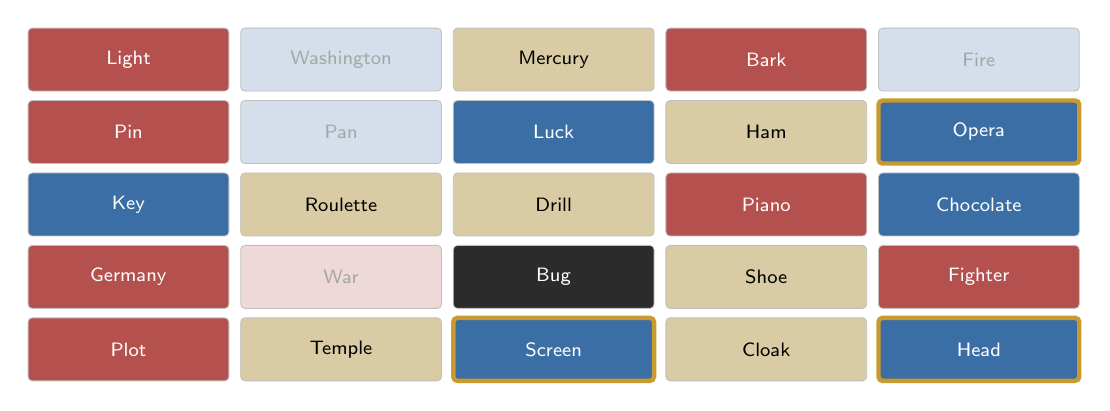
\begin{tikzpicture}[x=2.7cm, y=0.92cm]
  \node[draw=black!25, line width=0.3pt, fill=cnred, minimum width=2.55cm, minimum height=0.8cm, inner sep=1pt, rounded corners=1.5pt] at (0,0) {\textcolor{white}{\scriptsize\textsf{Light}}};
  \node[draw=black!25, line width=0.3pt, fill=cnblue!22, minimum width=2.55cm, minimum height=0.8cm, inner sep=1pt, rounded corners=1.5pt] at (1,0) {\textcolor{black!35}{\scriptsize\textsf{Washington}}};
  \node[draw=black!25, line width=0.3pt, fill=cntan, minimum width=2.55cm, minimum height=0.8cm, inner sep=1pt, rounded corners=1.5pt] at (2,0) {\textcolor{black}{\scriptsize\textsf{Mercury}}};
  \node[draw=black!25, line width=0.3pt, fill=cnred, minimum width=2.55cm, minimum height=0.8cm, inner sep=1pt, rounded corners=1.5pt] at (3,0) {\textcolor{white}{\scriptsize\textsf{Bark}}};
  \node[draw=black!25, line width=0.3pt, fill=cnblue!22, minimum width=2.55cm, minimum height=0.8cm, inner sep=1pt, rounded corners=1.5pt] at (4,0) {\textcolor{black!35}{\scriptsize\textsf{Fire}}};
  \node[draw=black!25, line width=0.3pt, fill=cnred, minimum width=2.55cm, minimum height=0.8cm, inner sep=1pt, rounded corners=1.5pt] at (0,-1) {\textcolor{white}{\scriptsize\textsf{Pin}}};
  \node[draw=black!25, line width=0.3pt, fill=cnblue!22, minimum width=2.55cm, minimum height=0.8cm, inner sep=1pt, rounded corners=1.5pt] at (1,-1) {\textcolor{black!35}{\scriptsize\textsf{Pan}}};
  \node[draw=black!25, line width=0.3pt, fill=cnblue, minimum width=2.55cm, minimum height=0.8cm, inner sep=1pt, rounded corners=1.5pt] at (2,-1) {\textcolor{white}{\scriptsize\textsf{Luck}}};
  \node[draw=black!25, line width=0.3pt, fill=cntan, minimum width=2.55cm, minimum height=0.8cm, inner sep=1pt, rounded corners=1.5pt] at (3,-1) {\textcolor{black}{\scriptsize\textsf{Ham}}};
  \node[draw=cngold, line width=1.6pt, fill=cnblue, minimum width=2.55cm, minimum height=0.8cm, inner sep=1pt, rounded corners=1.5pt] at (4,-1) {\textcolor{white}{\scriptsize\textsf{Opera}}};
  \node[draw=black!25, line width=0.3pt, fill=cnblue, minimum width=2.55cm, minimum height=0.8cm, inner sep=1pt, rounded corners=1.5pt] at (0,-2) {\textcolor{white}{\scriptsize\textsf{Key}}};
  \node[draw=black!25, line width=0.3pt, fill=cntan, minimum width=2.55cm, minimum height=0.8cm, inner sep=1pt, rounded corners=1.5pt] at (1,-2) {\textcolor{black}{\scriptsize\textsf{Roulette}}};
  \node[draw=black!25, line width=0.3pt, fill=cntan, minimum width=2.55cm, minimum height=0.8cm, inner sep=1pt, rounded corners=1.5pt] at (2,-2) {\textcolor{black}{\scriptsize\textsf{Drill}}};
  \node[draw=black!25, line width=0.3pt, fill=cnred, minimum width=2.55cm, minimum height=0.8cm, inner sep=1pt, rounded corners=1.5pt] at (3,-2) {\textcolor{white}{\scriptsize\textsf{Piano}}};
  \node[draw=black!25, line width=0.3pt, fill=cnblue, minimum width=2.55cm, minimum height=0.8cm, inner sep=1pt, rounded corners=1.5pt] at (4,-2) {\textcolor{white}{\scriptsize\textsf{Chocolate}}};
  \node[draw=black!25, line width=0.3pt, fill=cnred, minimum width=2.55cm, minimum height=0.8cm, inner sep=1pt, rounded corners=1.5pt] at (0,-3) {\textcolor{white}{\scriptsize\textsf{Germany}}};
  \node[draw=black!25, line width=0.3pt, fill=cnred!22, minimum width=2.55cm, minimum height=0.8cm, inner sep=1pt, rounded corners=1.5pt] at (1,-3) {\textcolor{black!35}{\scriptsize\textsf{War}}};
  \node[draw=black!25, line width=0.3pt, fill=cnblack, minimum width=2.55cm, minimum height=0.8cm, inner sep=1pt, rounded corners=1.5pt] at (2,-3) {\textcolor{white}{\scriptsize\textsf{Bug}}};
  \node[draw=black!25, line width=0.3pt, fill=cntan, minimum width=2.55cm, minimum height=0.8cm, inner sep=1pt, rounded corners=1.5pt] at (3,-3) {\textcolor{black}{\scriptsize\textsf{Shoe}}};
  \node[draw=black!25, line width=0.3pt, fill=cnred, minimum width=2.55cm, minimum height=0.8cm, inner sep=1pt, rounded corners=1.5pt] at (4,-3) {\textcolor{white}{\scriptsize\textsf{Fighter}}};
  \node[draw=black!25, line width=0.3pt, fill=cnred, minimum width=2.55cm, minimum height=0.8cm, inner sep=1pt, rounded corners=1.5pt] at (0,-4) {\textcolor{white}{\scriptsize\textsf{Plot}}};
  \node[draw=black!25, line width=0.3pt, fill=cntan, minimum width=2.55cm, minimum height=0.8cm, inner sep=1pt, rounded corners=1.5pt] at (1,-4) {\textcolor{black}{\scriptsize\textsf{Temple}}};
  \node[draw=cngold, line width=1.6pt, fill=cnblue, minimum width=2.55cm, minimum height=0.8cm, inner sep=1pt, rounded corners=1.5pt] at (2,-4) {\textcolor{white}{\scriptsize\textsf{Screen}}};
  \node[draw=black!25, line width=0.3pt, fill=cntan, minimum width=2.55cm, minimum height=0.8cm, inner sep=1pt, rounded corners=1.5pt] at (3,-4) {\textcolor{black}{\scriptsize\textsf{Cloak}}};
  \node[draw=cngold, line width=1.6pt, fill=cnblue, minimum width=2.55cm, minimum height=0.8cm, inner sep=1pt, rounded corners=1.5pt] at (4,-4) {\textcolor{white}{\scriptsize\textsf{Head}}};
\end{tikzpicture}
\caption*{\footnotesize \textbf{Turn 2} --- clue \textsc{directors} 3. Guesser took: \textbf{Screen}, Plot \textit{(opponent)}.}
\end{figure}

\begin{figure}[H]
\centering
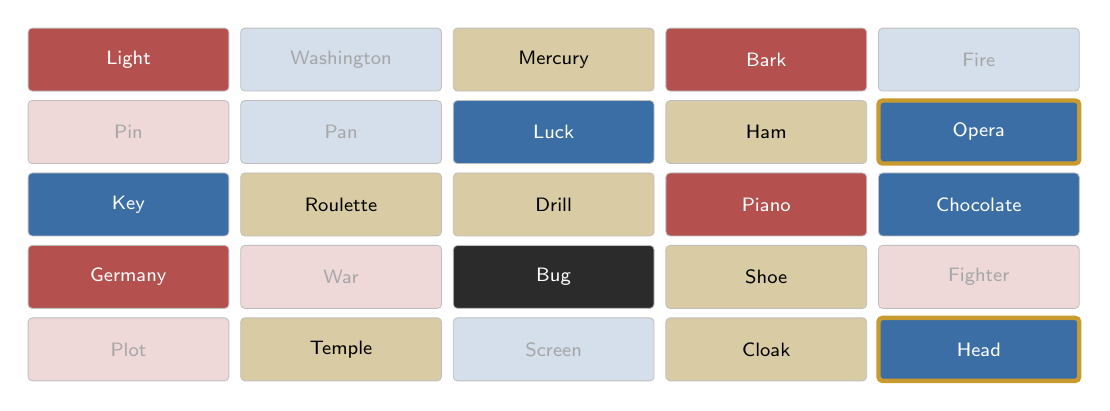
\begin{tikzpicture}[x=2.7cm, y=0.92cm]
  \node[draw=black!25, line width=0.3pt, fill=cnred, minimum width=2.55cm, minimum height=0.8cm, inner sep=1pt, rounded corners=1.5pt] at (0,0) {\textcolor{white}{\scriptsize\textsf{Light}}};
  \node[draw=black!25, line width=0.3pt, fill=cnblue!22, minimum width=2.55cm, minimum height=0.8cm, inner sep=1pt, rounded corners=1.5pt] at (1,0) {\textcolor{black!35}{\scriptsize\textsf{Washington}}};
  \node[draw=black!25, line width=0.3pt, fill=cntan, minimum width=2.55cm, minimum height=0.8cm, inner sep=1pt, rounded corners=1.5pt] at (2,0) {\textcolor{black}{\scriptsize\textsf{Mercury}}};
  \node[draw=black!25, line width=0.3pt, fill=cnred, minimum width=2.55cm, minimum height=0.8cm, inner sep=1pt, rounded corners=1.5pt] at (3,0) {\textcolor{white}{\scriptsize\textsf{Bark}}};
  \node[draw=black!25, line width=0.3pt, fill=cnblue!22, minimum width=2.55cm, minimum height=0.8cm, inner sep=1pt, rounded corners=1.5pt] at (4,0) {\textcolor{black!35}{\scriptsize\textsf{Fire}}};
  \node[draw=black!25, line width=0.3pt, fill=cnred!22, minimum width=2.55cm, minimum height=0.8cm, inner sep=1pt, rounded corners=1.5pt] at (0,-1) {\textcolor{black!35}{\scriptsize\textsf{Pin}}};
  \node[draw=black!25, line width=0.3pt, fill=cnblue!22, minimum width=2.55cm, minimum height=0.8cm, inner sep=1pt, rounded corners=1.5pt] at (1,-1) {\textcolor{black!35}{\scriptsize\textsf{Pan}}};
  \node[draw=black!25, line width=0.3pt, fill=cnblue, minimum width=2.55cm, minimum height=0.8cm, inner sep=1pt, rounded corners=1.5pt] at (2,-1) {\textcolor{white}{\scriptsize\textsf{Luck}}};
  \node[draw=black!25, line width=0.3pt, fill=cntan, minimum width=2.55cm, minimum height=0.8cm, inner sep=1pt, rounded corners=1.5pt] at (3,-1) {\textcolor{black}{\scriptsize\textsf{Ham}}};
  \node[draw=cngold, line width=1.6pt, fill=cnblue, minimum width=2.55cm, minimum height=0.8cm, inner sep=1pt, rounded corners=1.5pt] at (4,-1) {\textcolor{white}{\scriptsize\textsf{Opera}}};
  \node[draw=black!25, line width=0.3pt, fill=cnblue, minimum width=2.55cm, minimum height=0.8cm, inner sep=1pt, rounded corners=1.5pt] at (0,-2) {\textcolor{white}{\scriptsize\textsf{Key}}};
  \node[draw=black!25, line width=0.3pt, fill=cntan, minimum width=2.55cm, minimum height=0.8cm, inner sep=1pt, rounded corners=1.5pt] at (1,-2) {\textcolor{black}{\scriptsize\textsf{Roulette}}};
  \node[draw=black!25, line width=0.3pt, fill=cntan, minimum width=2.55cm, minimum height=0.8cm, inner sep=1pt, rounded corners=1.5pt] at (2,-2) {\textcolor{black}{\scriptsize\textsf{Drill}}};
  \node[draw=black!25, line width=0.3pt, fill=cnred, minimum width=2.55cm, minimum height=0.8cm, inner sep=1pt, rounded corners=1.5pt] at (3,-2) {\textcolor{white}{\scriptsize\textsf{Piano}}};
  \node[draw=black!25, line width=0.3pt, fill=cnblue, minimum width=2.55cm, minimum height=0.8cm, inner sep=1pt, rounded corners=1.5pt] at (4,-2) {\textcolor{white}{\scriptsize\textsf{Chocolate}}};
  \node[draw=black!25, line width=0.3pt, fill=cnred, minimum width=2.55cm, minimum height=0.8cm, inner sep=1pt, rounded corners=1.5pt] at (0,-3) {\textcolor{white}{\scriptsize\textsf{Germany}}};
  \node[draw=black!25, line width=0.3pt, fill=cnred!22, minimum width=2.55cm, minimum height=0.8cm, inner sep=1pt, rounded corners=1.5pt] at (1,-3) {\textcolor{black!35}{\scriptsize\textsf{War}}};
  \node[draw=black!25, line width=0.3pt, fill=cnblack, minimum width=2.55cm, minimum height=0.8cm, inner sep=1pt, rounded corners=1.5pt] at (2,-3) {\textcolor{white}{\scriptsize\textsf{Bug}}};
  \node[draw=black!25, line width=0.3pt, fill=cntan, minimum width=2.55cm, minimum height=0.8cm, inner sep=1pt, rounded corners=1.5pt] at (3,-3) {\textcolor{black}{\scriptsize\textsf{Shoe}}};
  \node[draw=black!25, line width=0.3pt, fill=cnred!22, minimum width=2.55cm, minimum height=0.8cm, inner sep=1pt, rounded corners=1.5pt] at (4,-3) {\textcolor{black!35}{\scriptsize\textsf{Fighter}}};
  \node[draw=black!25, line width=0.3pt, fill=cnred!22, minimum width=2.55cm, minimum height=0.8cm, inner sep=1pt, rounded corners=1.5pt] at (0,-4) {\textcolor{black!35}{\scriptsize\textsf{Plot}}};
  \node[draw=black!25, line width=0.3pt, fill=cntan, minimum width=2.55cm, minimum height=0.8cm, inner sep=1pt, rounded corners=1.5pt] at (1,-4) {\textcolor{black}{\scriptsize\textsf{Temple}}};
  \node[draw=black!25, line width=0.3pt, fill=cnblue!22, minimum width=2.55cm, minimum height=0.8cm, inner sep=1pt, rounded corners=1.5pt] at (2,-4) {\textcolor{black!35}{\scriptsize\textsf{Screen}}};
  \node[draw=black!25, line width=0.3pt, fill=cntan, minimum width=2.55cm, minimum height=0.8cm, inner sep=1pt, rounded corners=1.5pt] at (3,-4) {\textcolor{black}{\scriptsize\textsf{Cloak}}};
  \node[draw=cngold, line width=1.6pt, fill=cnblue, minimum width=2.55cm, minimum height=0.8cm, inner sep=1pt, rounded corners=1.5pt] at (4,-4) {\textcolor{white}{\scriptsize\textsf{Head}}};
\end{tikzpicture}
\caption*{\footnotesize \textbf{Turn 3} --- clue \textsc{directors} 2. Guesser took: \textbf{Opera}, \textbf{Head}.}
\end{figure}

\begin{figure}[H]
\centering
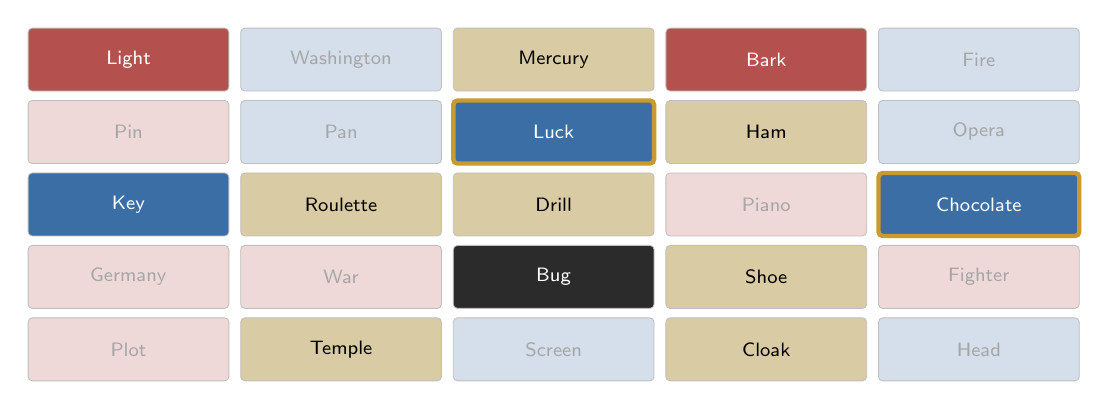
\begin{tikzpicture}[x=2.7cm, y=0.92cm]
  \node[draw=black!25, line width=0.3pt, fill=cnred, minimum width=2.55cm, minimum height=0.8cm, inner sep=1pt, rounded corners=1.5pt] at (0,0) {\textcolor{white}{\scriptsize\textsf{Light}}};
  \node[draw=black!25, line width=0.3pt, fill=cnblue!22, minimum width=2.55cm, minimum height=0.8cm, inner sep=1pt, rounded corners=1.5pt] at (1,0) {\textcolor{black!35}{\scriptsize\textsf{Washington}}};
  \node[draw=black!25, line width=0.3pt, fill=cntan, minimum width=2.55cm, minimum height=0.8cm, inner sep=1pt, rounded corners=1.5pt] at (2,0) {\textcolor{black}{\scriptsize\textsf{Mercury}}};
  \node[draw=black!25, line width=0.3pt, fill=cnred, minimum width=2.55cm, minimum height=0.8cm, inner sep=1pt, rounded corners=1.5pt] at (3,0) {\textcolor{white}{\scriptsize\textsf{Bark}}};
  \node[draw=black!25, line width=0.3pt, fill=cnblue!22, minimum width=2.55cm, minimum height=0.8cm, inner sep=1pt, rounded corners=1.5pt] at (4,0) {\textcolor{black!35}{\scriptsize\textsf{Fire}}};
  \node[draw=black!25, line width=0.3pt, fill=cnred!22, minimum width=2.55cm, minimum height=0.8cm, inner sep=1pt, rounded corners=1.5pt] at (0,-1) {\textcolor{black!35}{\scriptsize\textsf{Pin}}};
  \node[draw=black!25, line width=0.3pt, fill=cnblue!22, minimum width=2.55cm, minimum height=0.8cm, inner sep=1pt, rounded corners=1.5pt] at (1,-1) {\textcolor{black!35}{\scriptsize\textsf{Pan}}};
  \node[draw=cngold, line width=1.6pt, fill=cnblue, minimum width=2.55cm, minimum height=0.8cm, inner sep=1pt, rounded corners=1.5pt] at (2,-1) {\textcolor{white}{\scriptsize\textsf{Luck}}};
  \node[draw=black!25, line width=0.3pt, fill=cntan, minimum width=2.55cm, minimum height=0.8cm, inner sep=1pt, rounded corners=1.5pt] at (3,-1) {\textcolor{black}{\scriptsize\textsf{Ham}}};
  \node[draw=black!25, line width=0.3pt, fill=cnblue!22, minimum width=2.55cm, minimum height=0.8cm, inner sep=1pt, rounded corners=1.5pt] at (4,-1) {\textcolor{black!35}{\scriptsize\textsf{Opera}}};
  \node[draw=black!25, line width=0.3pt, fill=cnblue, minimum width=2.55cm, minimum height=0.8cm, inner sep=1pt, rounded corners=1.5pt] at (0,-2) {\textcolor{white}{\scriptsize\textsf{Key}}};
  \node[draw=black!25, line width=0.3pt, fill=cntan, minimum width=2.55cm, minimum height=0.8cm, inner sep=1pt, rounded corners=1.5pt] at (1,-2) {\textcolor{black}{\scriptsize\textsf{Roulette}}};
  \node[draw=black!25, line width=0.3pt, fill=cntan, minimum width=2.55cm, minimum height=0.8cm, inner sep=1pt, rounded corners=1.5pt] at (2,-2) {\textcolor{black}{\scriptsize\textsf{Drill}}};
  \node[draw=black!25, line width=0.3pt, fill=cnred!22, minimum width=2.55cm, minimum height=0.8cm, inner sep=1pt, rounded corners=1.5pt] at (3,-2) {\textcolor{black!35}{\scriptsize\textsf{Piano}}};
  \node[draw=cngold, line width=1.6pt, fill=cnblue, minimum width=2.55cm, minimum height=0.8cm, inner sep=1pt, rounded corners=1.5pt] at (4,-2) {\textcolor{white}{\scriptsize\textsf{Chocolate}}};
  \node[draw=black!25, line width=0.3pt, fill=cnred!22, minimum width=2.55cm, minimum height=0.8cm, inner sep=1pt, rounded corners=1.5pt] at (0,-3) {\textcolor{black!35}{\scriptsize\textsf{Germany}}};
  \node[draw=black!25, line width=0.3pt, fill=cnred!22, minimum width=2.55cm, minimum height=0.8cm, inner sep=1pt, rounded corners=1.5pt] at (1,-3) {\textcolor{black!35}{\scriptsize\textsf{War}}};
  \node[draw=black!25, line width=0.3pt, fill=cnblack, minimum width=2.55cm, minimum height=0.8cm, inner sep=1pt, rounded corners=1.5pt] at (2,-3) {\textcolor{white}{\scriptsize\textsf{Bug}}};
  \node[draw=black!25, line width=0.3pt, fill=cntan, minimum width=2.55cm, minimum height=0.8cm, inner sep=1pt, rounded corners=1.5pt] at (3,-3) {\textcolor{black}{\scriptsize\textsf{Shoe}}};
  \node[draw=black!25, line width=0.3pt, fill=cnred!22, minimum width=2.55cm, minimum height=0.8cm, inner sep=1pt, rounded corners=1.5pt] at (4,-3) {\textcolor{black!35}{\scriptsize\textsf{Fighter}}};
  \node[draw=black!25, line width=0.3pt, fill=cnred!22, minimum width=2.55cm, minimum height=0.8cm, inner sep=1pt, rounded corners=1.5pt] at (0,-4) {\textcolor{black!35}{\scriptsize\textsf{Plot}}};
  \node[draw=black!25, line width=0.3pt, fill=cntan, minimum width=2.55cm, minimum height=0.8cm, inner sep=1pt, rounded corners=1.5pt] at (1,-4) {\textcolor{black}{\scriptsize\textsf{Temple}}};
  \node[draw=black!25, line width=0.3pt, fill=cnblue!22, minimum width=2.55cm, minimum height=0.8cm, inner sep=1pt, rounded corners=1.5pt] at (2,-4) {\textcolor{black!35}{\scriptsize\textsf{Screen}}};
  \node[draw=black!25, line width=0.3pt, fill=cntan, minimum width=2.55cm, minimum height=0.8cm, inner sep=1pt, rounded corners=1.5pt] at (3,-4) {\textcolor{black}{\scriptsize\textsf{Cloak}}};
  \node[draw=black!25, line width=0.3pt, fill=cnblue!22, minimum width=2.55cm, minimum height=0.8cm, inner sep=1pt, rounded corners=1.5pt] at (4,-4) {\textcolor{black!35}{\scriptsize\textsf{Head}}};
\end{tikzpicture}
\caption*{\footnotesize \textbf{Turn 4} --- clue \textsc{good} 2. Guesser took: \textbf{Luck}, \textbf{Chocolate}.}
\end{figure}


\clearpage

\section*{Game 3}

\begin{figure}[H]
\centering
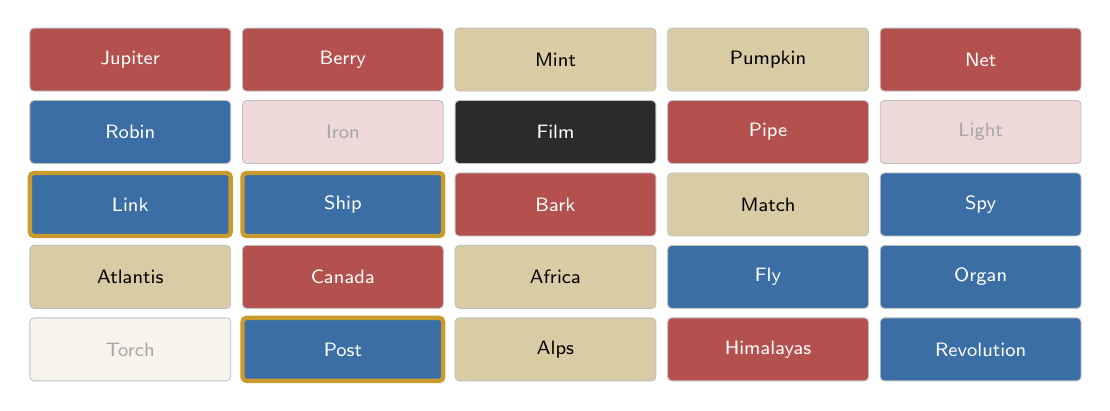
\begin{tikzpicture}[x=2.7cm, y=0.92cm]
  \node[draw=black!25, line width=0.3pt, fill=cnred, minimum width=2.55cm, minimum height=0.8cm, inner sep=1pt, rounded corners=1.5pt] at (0,0) {\textcolor{white}{\scriptsize\textsf{Jupiter}}};
  \node[draw=black!25, line width=0.3pt, fill=cnred, minimum width=2.55cm, minimum height=0.8cm, inner sep=1pt, rounded corners=1.5pt] at (1,0) {\textcolor{white}{\scriptsize\textsf{Berry}}};
  \node[draw=black!25, line width=0.3pt, fill=cntan, minimum width=2.55cm, minimum height=0.8cm, inner sep=1pt, rounded corners=1.5pt] at (2,0) {\textcolor{black}{\scriptsize\textsf{Mint}}};
  \node[draw=black!25, line width=0.3pt, fill=cntan, minimum width=2.55cm, minimum height=0.8cm, inner sep=1pt, rounded corners=1.5pt] at (3,0) {\textcolor{black}{\scriptsize\textsf{Pumpkin}}};
  \node[draw=black!25, line width=0.3pt, fill=cnred, minimum width=2.55cm, minimum height=0.8cm, inner sep=1pt, rounded corners=1.5pt] at (4,0) {\textcolor{white}{\scriptsize\textsf{Net}}};
  \node[draw=black!25, line width=0.3pt, fill=cnblue, minimum width=2.55cm, minimum height=0.8cm, inner sep=1pt, rounded corners=1.5pt] at (0,-1) {\textcolor{white}{\scriptsize\textsf{Robin}}};
  \node[draw=black!25, line width=0.3pt, fill=cnred!22, minimum width=2.55cm, minimum height=0.8cm, inner sep=1pt, rounded corners=1.5pt] at (1,-1) {\textcolor{black!35}{\scriptsize\textsf{Iron}}};
  \node[draw=black!25, line width=0.3pt, fill=cnblack, minimum width=2.55cm, minimum height=0.8cm, inner sep=1pt, rounded corners=1.5pt] at (2,-1) {\textcolor{white}{\scriptsize\textsf{Film}}};
  \node[draw=black!25, line width=0.3pt, fill=cnred, minimum width=2.55cm, minimum height=0.8cm, inner sep=1pt, rounded corners=1.5pt] at (3,-1) {\textcolor{white}{\scriptsize\textsf{Pipe}}};
  \node[draw=black!25, line width=0.3pt, fill=cnred!22, minimum width=2.55cm, minimum height=0.8cm, inner sep=1pt, rounded corners=1.5pt] at (4,-1) {\textcolor{black!35}{\scriptsize\textsf{Light}}};
  \node[draw=cngold, line width=1.6pt, fill=cnblue, minimum width=2.55cm, minimum height=0.8cm, inner sep=1pt, rounded corners=1.5pt] at (0,-2) {\textcolor{white}{\scriptsize\textsf{Link}}};
  \node[draw=cngold, line width=1.6pt, fill=cnblue, minimum width=2.55cm, minimum height=0.8cm, inner sep=1pt, rounded corners=1.5pt] at (1,-2) {\textcolor{white}{\scriptsize\textsf{Ship}}};
  \node[draw=black!25, line width=0.3pt, fill=cnred, minimum width=2.55cm, minimum height=0.8cm, inner sep=1pt, rounded corners=1.5pt] at (2,-2) {\textcolor{white}{\scriptsize\textsf{Bark}}};
  \node[draw=black!25, line width=0.3pt, fill=cntan, minimum width=2.55cm, minimum height=0.8cm, inner sep=1pt, rounded corners=1.5pt] at (3,-2) {\textcolor{black}{\scriptsize\textsf{Match}}};
  \node[draw=black!25, line width=0.3pt, fill=cnblue, minimum width=2.55cm, minimum height=0.8cm, inner sep=1pt, rounded corners=1.5pt] at (4,-2) {\textcolor{white}{\scriptsize\textsf{Spy}}};
  \node[draw=black!25, line width=0.3pt, fill=cntan, minimum width=2.55cm, minimum height=0.8cm, inner sep=1pt, rounded corners=1.5pt] at (0,-3) {\textcolor{black}{\scriptsize\textsf{Atlantis}}};
  \node[draw=black!25, line width=0.3pt, fill=cnred, minimum width=2.55cm, minimum height=0.8cm, inner sep=1pt, rounded corners=1.5pt] at (1,-3) {\textcolor{white}{\scriptsize\textsf{Canada}}};
  \node[draw=black!25, line width=0.3pt, fill=cntan, minimum width=2.55cm, minimum height=0.8cm, inner sep=1pt, rounded corners=1.5pt] at (2,-3) {\textcolor{black}{\scriptsize\textsf{Africa}}};
  \node[draw=black!25, line width=0.3pt, fill=cnblue, minimum width=2.55cm, minimum height=0.8cm, inner sep=1pt, rounded corners=1.5pt] at (3,-3) {\textcolor{white}{\scriptsize\textsf{Fly}}};
  \node[draw=black!25, line width=0.3pt, fill=cnblue, minimum width=2.55cm, minimum height=0.8cm, inner sep=1pt, rounded corners=1.5pt] at (4,-3) {\textcolor{white}{\scriptsize\textsf{Organ}}};
  \node[draw=black!25, line width=0.3pt, fill=cntan!22, minimum width=2.55cm, minimum height=0.8cm, inner sep=1pt, rounded corners=1.5pt] at (0,-4) {\textcolor{black!35}{\scriptsize\textsf{Torch}}};
  \node[draw=cngold, line width=1.6pt, fill=cnblue, minimum width=2.55cm, minimum height=0.8cm, inner sep=1pt, rounded corners=1.5pt] at (1,-4) {\textcolor{white}{\scriptsize\textsf{Post}}};
  \node[draw=black!25, line width=0.3pt, fill=cntan, minimum width=2.55cm, minimum height=0.8cm, inner sep=1pt, rounded corners=1.5pt] at (2,-4) {\textcolor{black}{\scriptsize\textsf{Alps}}};
  \node[draw=black!25, line width=0.3pt, fill=cnred, minimum width=2.55cm, minimum height=0.8cm, inner sep=1pt, rounded corners=1.5pt] at (3,-4) {\textcolor{white}{\scriptsize\textsf{Himalayas}}};
  \node[draw=black!25, line width=0.3pt, fill=cnblue, minimum width=2.55cm, minimum height=0.8cm, inner sep=1pt, rounded corners=1.5pt] at (4,-4) {\textcolor{white}{\scriptsize\textsf{Revolution}}};
\end{tikzpicture}
\caption*{\footnotesize \textbf{Turn 1} --- clue \textsc{send} 3. Guesser took: \textbf{Ship}, \textbf{Post}, \textbf{Link}.}
\end{figure}

\begin{figure}[H]
\centering
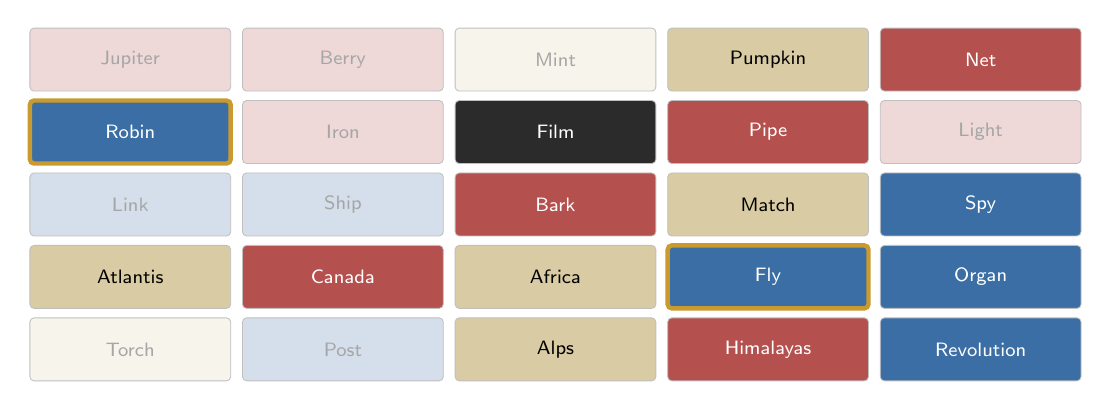
\begin{tikzpicture}[x=2.7cm, y=0.92cm]
  \node[draw=black!25, line width=0.3pt, fill=cnred!22, minimum width=2.55cm, minimum height=0.8cm, inner sep=1pt, rounded corners=1.5pt] at (0,0) {\textcolor{black!35}{\scriptsize\textsf{Jupiter}}};
  \node[draw=black!25, line width=0.3pt, fill=cnred!22, minimum width=2.55cm, minimum height=0.8cm, inner sep=1pt, rounded corners=1.5pt] at (1,0) {\textcolor{black!35}{\scriptsize\textsf{Berry}}};
  \node[draw=black!25, line width=0.3pt, fill=cntan!22, minimum width=2.55cm, minimum height=0.8cm, inner sep=1pt, rounded corners=1.5pt] at (2,0) {\textcolor{black!35}{\scriptsize\textsf{Mint}}};
  \node[draw=black!25, line width=0.3pt, fill=cntan, minimum width=2.55cm, minimum height=0.8cm, inner sep=1pt, rounded corners=1.5pt] at (3,0) {\textcolor{black}{\scriptsize\textsf{Pumpkin}}};
  \node[draw=black!25, line width=0.3pt, fill=cnred, minimum width=2.55cm, minimum height=0.8cm, inner sep=1pt, rounded corners=1.5pt] at (4,0) {\textcolor{white}{\scriptsize\textsf{Net}}};
  \node[draw=cngold, line width=1.6pt, fill=cnblue, minimum width=2.55cm, minimum height=0.8cm, inner sep=1pt, rounded corners=1.5pt] at (0,-1) {\textcolor{white}{\scriptsize\textsf{Robin}}};
  \node[draw=black!25, line width=0.3pt, fill=cnred!22, minimum width=2.55cm, minimum height=0.8cm, inner sep=1pt, rounded corners=1.5pt] at (1,-1) {\textcolor{black!35}{\scriptsize\textsf{Iron}}};
  \node[draw=black!25, line width=0.3pt, fill=cnblack, minimum width=2.55cm, minimum height=0.8cm, inner sep=1pt, rounded corners=1.5pt] at (2,-1) {\textcolor{white}{\scriptsize\textsf{Film}}};
  \node[draw=black!25, line width=0.3pt, fill=cnred, minimum width=2.55cm, minimum height=0.8cm, inner sep=1pt, rounded corners=1.5pt] at (3,-1) {\textcolor{white}{\scriptsize\textsf{Pipe}}};
  \node[draw=black!25, line width=0.3pt, fill=cnred!22, minimum width=2.55cm, minimum height=0.8cm, inner sep=1pt, rounded corners=1.5pt] at (4,-1) {\textcolor{black!35}{\scriptsize\textsf{Light}}};
  \node[draw=black!25, line width=0.3pt, fill=cnblue!22, minimum width=2.55cm, minimum height=0.8cm, inner sep=1pt, rounded corners=1.5pt] at (0,-2) {\textcolor{black!35}{\scriptsize\textsf{Link}}};
  \node[draw=black!25, line width=0.3pt, fill=cnblue!22, minimum width=2.55cm, minimum height=0.8cm, inner sep=1pt, rounded corners=1.5pt] at (1,-2) {\textcolor{black!35}{\scriptsize\textsf{Ship}}};
  \node[draw=black!25, line width=0.3pt, fill=cnred, minimum width=2.55cm, minimum height=0.8cm, inner sep=1pt, rounded corners=1.5pt] at (2,-2) {\textcolor{white}{\scriptsize\textsf{Bark}}};
  \node[draw=black!25, line width=0.3pt, fill=cntan, minimum width=2.55cm, minimum height=0.8cm, inner sep=1pt, rounded corners=1.5pt] at (3,-2) {\textcolor{black}{\scriptsize\textsf{Match}}};
  \node[draw=black!25, line width=0.3pt, fill=cnblue, minimum width=2.55cm, minimum height=0.8cm, inner sep=1pt, rounded corners=1.5pt] at (4,-2) {\textcolor{white}{\scriptsize\textsf{Spy}}};
  \node[draw=black!25, line width=0.3pt, fill=cntan, minimum width=2.55cm, minimum height=0.8cm, inner sep=1pt, rounded corners=1.5pt] at (0,-3) {\textcolor{black}{\scriptsize\textsf{Atlantis}}};
  \node[draw=black!25, line width=0.3pt, fill=cnred, minimum width=2.55cm, minimum height=0.8cm, inner sep=1pt, rounded corners=1.5pt] at (1,-3) {\textcolor{white}{\scriptsize\textsf{Canada}}};
  \node[draw=black!25, line width=0.3pt, fill=cntan, minimum width=2.55cm, minimum height=0.8cm, inner sep=1pt, rounded corners=1.5pt] at (2,-3) {\textcolor{black}{\scriptsize\textsf{Africa}}};
  \node[draw=cngold, line width=1.6pt, fill=cnblue, minimum width=2.55cm, minimum height=0.8cm, inner sep=1pt, rounded corners=1.5pt] at (3,-3) {\textcolor{white}{\scriptsize\textsf{Fly}}};
  \node[draw=black!25, line width=0.3pt, fill=cnblue, minimum width=2.55cm, minimum height=0.8cm, inner sep=1pt, rounded corners=1.5pt] at (4,-3) {\textcolor{white}{\scriptsize\textsf{Organ}}};
  \node[draw=black!25, line width=0.3pt, fill=cntan!22, minimum width=2.55cm, minimum height=0.8cm, inner sep=1pt, rounded corners=1.5pt] at (0,-4) {\textcolor{black!35}{\scriptsize\textsf{Torch}}};
  \node[draw=black!25, line width=0.3pt, fill=cnblue!22, minimum width=2.55cm, minimum height=0.8cm, inner sep=1pt, rounded corners=1.5pt] at (1,-4) {\textcolor{black!35}{\scriptsize\textsf{Post}}};
  \node[draw=black!25, line width=0.3pt, fill=cntan, minimum width=2.55cm, minimum height=0.8cm, inner sep=1pt, rounded corners=1.5pt] at (2,-4) {\textcolor{black}{\scriptsize\textsf{Alps}}};
  \node[draw=black!25, line width=0.3pt, fill=cnred, minimum width=2.55cm, minimum height=0.8cm, inner sep=1pt, rounded corners=1.5pt] at (3,-4) {\textcolor{white}{\scriptsize\textsf{Himalayas}}};
  \node[draw=black!25, line width=0.3pt, fill=cnblue, minimum width=2.55cm, minimum height=0.8cm, inner sep=1pt, rounded corners=1.5pt] at (4,-4) {\textcolor{white}{\scriptsize\textsf{Revolution}}};
\end{tikzpicture}
\caption*{\footnotesize \textbf{Turn 2} --- clue \textsc{bird} 2. Guesser took: \textbf{Robin}, \textbf{Fly}.}
\end{figure}

\begin{figure}[H]
\centering
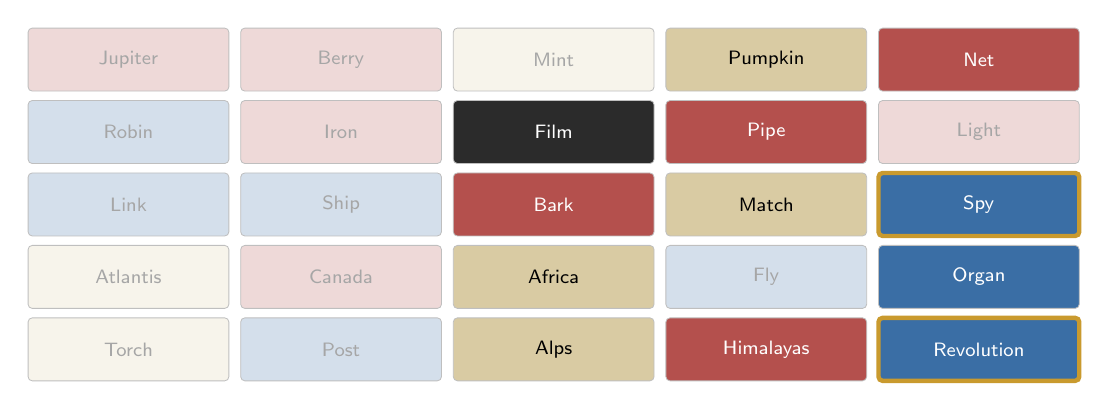
\begin{tikzpicture}[x=2.7cm, y=0.92cm]
  \node[draw=black!25, line width=0.3pt, fill=cnred!22, minimum width=2.55cm, minimum height=0.8cm, inner sep=1pt, rounded corners=1.5pt] at (0,0) {\textcolor{black!35}{\scriptsize\textsf{Jupiter}}};
  \node[draw=black!25, line width=0.3pt, fill=cnred!22, minimum width=2.55cm, minimum height=0.8cm, inner sep=1pt, rounded corners=1.5pt] at (1,0) {\textcolor{black!35}{\scriptsize\textsf{Berry}}};
  \node[draw=black!25, line width=0.3pt, fill=cntan!22, minimum width=2.55cm, minimum height=0.8cm, inner sep=1pt, rounded corners=1.5pt] at (2,0) {\textcolor{black!35}{\scriptsize\textsf{Mint}}};
  \node[draw=black!25, line width=0.3pt, fill=cntan, minimum width=2.55cm, minimum height=0.8cm, inner sep=1pt, rounded corners=1.5pt] at (3,0) {\textcolor{black}{\scriptsize\textsf{Pumpkin}}};
  \node[draw=black!25, line width=0.3pt, fill=cnred, minimum width=2.55cm, minimum height=0.8cm, inner sep=1pt, rounded corners=1.5pt] at (4,0) {\textcolor{white}{\scriptsize\textsf{Net}}};
  \node[draw=black!25, line width=0.3pt, fill=cnblue!22, minimum width=2.55cm, minimum height=0.8cm, inner sep=1pt, rounded corners=1.5pt] at (0,-1) {\textcolor{black!35}{\scriptsize\textsf{Robin}}};
  \node[draw=black!25, line width=0.3pt, fill=cnred!22, minimum width=2.55cm, minimum height=0.8cm, inner sep=1pt, rounded corners=1.5pt] at (1,-1) {\textcolor{black!35}{\scriptsize\textsf{Iron}}};
  \node[draw=black!25, line width=0.3pt, fill=cnblack, minimum width=2.55cm, minimum height=0.8cm, inner sep=1pt, rounded corners=1.5pt] at (2,-1) {\textcolor{white}{\scriptsize\textsf{Film}}};
  \node[draw=black!25, line width=0.3pt, fill=cnred, minimum width=2.55cm, minimum height=0.8cm, inner sep=1pt, rounded corners=1.5pt] at (3,-1) {\textcolor{white}{\scriptsize\textsf{Pipe}}};
  \node[draw=black!25, line width=0.3pt, fill=cnred!22, minimum width=2.55cm, minimum height=0.8cm, inner sep=1pt, rounded corners=1.5pt] at (4,-1) {\textcolor{black!35}{\scriptsize\textsf{Light}}};
  \node[draw=black!25, line width=0.3pt, fill=cnblue!22, minimum width=2.55cm, minimum height=0.8cm, inner sep=1pt, rounded corners=1.5pt] at (0,-2) {\textcolor{black!35}{\scriptsize\textsf{Link}}};
  \node[draw=black!25, line width=0.3pt, fill=cnblue!22, minimum width=2.55cm, minimum height=0.8cm, inner sep=1pt, rounded corners=1.5pt] at (1,-2) {\textcolor{black!35}{\scriptsize\textsf{Ship}}};
  \node[draw=black!25, line width=0.3pt, fill=cnred, minimum width=2.55cm, minimum height=0.8cm, inner sep=1pt, rounded corners=1.5pt] at (2,-2) {\textcolor{white}{\scriptsize\textsf{Bark}}};
  \node[draw=black!25, line width=0.3pt, fill=cntan, minimum width=2.55cm, minimum height=0.8cm, inner sep=1pt, rounded corners=1.5pt] at (3,-2) {\textcolor{black}{\scriptsize\textsf{Match}}};
  \node[draw=cngold, line width=1.6pt, fill=cnblue, minimum width=2.55cm, minimum height=0.8cm, inner sep=1pt, rounded corners=1.5pt] at (4,-2) {\textcolor{white}{\scriptsize\textsf{Spy}}};
  \node[draw=black!25, line width=0.3pt, fill=cntan!22, minimum width=2.55cm, minimum height=0.8cm, inner sep=1pt, rounded corners=1.5pt] at (0,-3) {\textcolor{black!35}{\scriptsize\textsf{Atlantis}}};
  \node[draw=black!25, line width=0.3pt, fill=cnred!22, minimum width=2.55cm, minimum height=0.8cm, inner sep=1pt, rounded corners=1.5pt] at (1,-3) {\textcolor{black!35}{\scriptsize\textsf{Canada}}};
  \node[draw=black!25, line width=0.3pt, fill=cntan, minimum width=2.55cm, minimum height=0.8cm, inner sep=1pt, rounded corners=1.5pt] at (2,-3) {\textcolor{black}{\scriptsize\textsf{Africa}}};
  \node[draw=black!25, line width=0.3pt, fill=cnblue!22, minimum width=2.55cm, minimum height=0.8cm, inner sep=1pt, rounded corners=1.5pt] at (3,-3) {\textcolor{black!35}{\scriptsize\textsf{Fly}}};
  \node[draw=black!25, line width=0.3pt, fill=cnblue, minimum width=2.55cm, minimum height=0.8cm, inner sep=1pt, rounded corners=1.5pt] at (4,-3) {\textcolor{white}{\scriptsize\textsf{Organ}}};
  \node[draw=black!25, line width=0.3pt, fill=cntan!22, minimum width=2.55cm, minimum height=0.8cm, inner sep=1pt, rounded corners=1.5pt] at (0,-4) {\textcolor{black!35}{\scriptsize\textsf{Torch}}};
  \node[draw=black!25, line width=0.3pt, fill=cnblue!22, minimum width=2.55cm, minimum height=0.8cm, inner sep=1pt, rounded corners=1.5pt] at (1,-4) {\textcolor{black!35}{\scriptsize\textsf{Post}}};
  \node[draw=black!25, line width=0.3pt, fill=cntan, minimum width=2.55cm, minimum height=0.8cm, inner sep=1pt, rounded corners=1.5pt] at (2,-4) {\textcolor{black}{\scriptsize\textsf{Alps}}};
  \node[draw=black!25, line width=0.3pt, fill=cnred, minimum width=2.55cm, minimum height=0.8cm, inner sep=1pt, rounded corners=1.5pt] at (3,-4) {\textcolor{white}{\scriptsize\textsf{Himalayas}}};
  \node[draw=cngold, line width=1.6pt, fill=cnblue, minimum width=2.55cm, minimum height=0.8cm, inner sep=1pt, rounded corners=1.5pt] at (4,-4) {\textcolor{white}{\scriptsize\textsf{Revolution}}};
\end{tikzpicture}
\caption*{\footnotesize \textbf{Turn 3} --- clue \textsc{treason} 2. Guesser took: \textbf{Spy}, \textbf{Revolution}.}
\end{figure}

\begin{figure}[H]
\centering
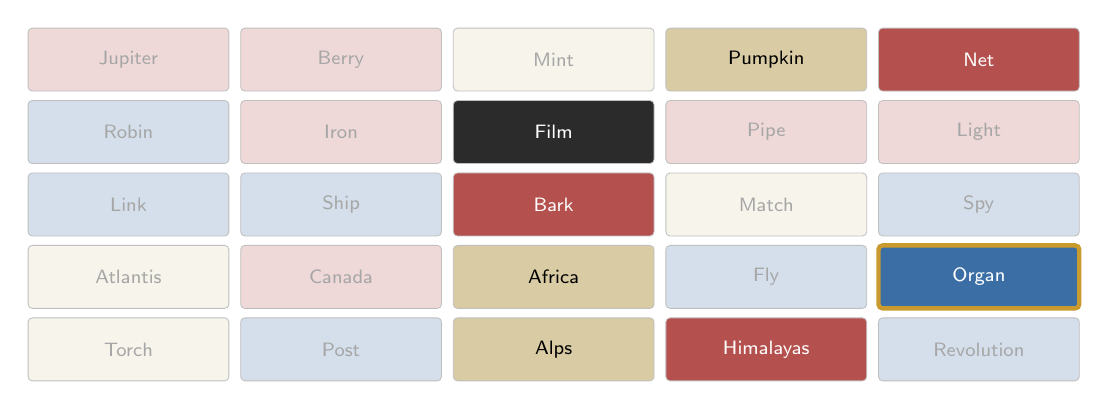
\begin{tikzpicture}[x=2.7cm, y=0.92cm]
  \node[draw=black!25, line width=0.3pt, fill=cnred!22, minimum width=2.55cm, minimum height=0.8cm, inner sep=1pt, rounded corners=1.5pt] at (0,0) {\textcolor{black!35}{\scriptsize\textsf{Jupiter}}};
  \node[draw=black!25, line width=0.3pt, fill=cnred!22, minimum width=2.55cm, minimum height=0.8cm, inner sep=1pt, rounded corners=1.5pt] at (1,0) {\textcolor{black!35}{\scriptsize\textsf{Berry}}};
  \node[draw=black!25, line width=0.3pt, fill=cntan!22, minimum width=2.55cm, minimum height=0.8cm, inner sep=1pt, rounded corners=1.5pt] at (2,0) {\textcolor{black!35}{\scriptsize\textsf{Mint}}};
  \node[draw=black!25, line width=0.3pt, fill=cntan, minimum width=2.55cm, minimum height=0.8cm, inner sep=1pt, rounded corners=1.5pt] at (3,0) {\textcolor{black}{\scriptsize\textsf{Pumpkin}}};
  \node[draw=black!25, line width=0.3pt, fill=cnred, minimum width=2.55cm, minimum height=0.8cm, inner sep=1pt, rounded corners=1.5pt] at (4,0) {\textcolor{white}{\scriptsize\textsf{Net}}};
  \node[draw=black!25, line width=0.3pt, fill=cnblue!22, minimum width=2.55cm, minimum height=0.8cm, inner sep=1pt, rounded corners=1.5pt] at (0,-1) {\textcolor{black!35}{\scriptsize\textsf{Robin}}};
  \node[draw=black!25, line width=0.3pt, fill=cnred!22, minimum width=2.55cm, minimum height=0.8cm, inner sep=1pt, rounded corners=1.5pt] at (1,-1) {\textcolor{black!35}{\scriptsize\textsf{Iron}}};
  \node[draw=black!25, line width=0.3pt, fill=cnblack, minimum width=2.55cm, minimum height=0.8cm, inner sep=1pt, rounded corners=1.5pt] at (2,-1) {\textcolor{white}{\scriptsize\textsf{Film}}};
  \node[draw=black!25, line width=0.3pt, fill=cnred!22, minimum width=2.55cm, minimum height=0.8cm, inner sep=1pt, rounded corners=1.5pt] at (3,-1) {\textcolor{black!35}{\scriptsize\textsf{Pipe}}};
  \node[draw=black!25, line width=0.3pt, fill=cnred!22, minimum width=2.55cm, minimum height=0.8cm, inner sep=1pt, rounded corners=1.5pt] at (4,-1) {\textcolor{black!35}{\scriptsize\textsf{Light}}};
  \node[draw=black!25, line width=0.3pt, fill=cnblue!22, minimum width=2.55cm, minimum height=0.8cm, inner sep=1pt, rounded corners=1.5pt] at (0,-2) {\textcolor{black!35}{\scriptsize\textsf{Link}}};
  \node[draw=black!25, line width=0.3pt, fill=cnblue!22, minimum width=2.55cm, minimum height=0.8cm, inner sep=1pt, rounded corners=1.5pt] at (1,-2) {\textcolor{black!35}{\scriptsize\textsf{Ship}}};
  \node[draw=black!25, line width=0.3pt, fill=cnred, minimum width=2.55cm, minimum height=0.8cm, inner sep=1pt, rounded corners=1.5pt] at (2,-2) {\textcolor{white}{\scriptsize\textsf{Bark}}};
  \node[draw=black!25, line width=0.3pt, fill=cntan!22, minimum width=2.55cm, minimum height=0.8cm, inner sep=1pt, rounded corners=1.5pt] at (3,-2) {\textcolor{black!35}{\scriptsize\textsf{Match}}};
  \node[draw=black!25, line width=0.3pt, fill=cnblue!22, minimum width=2.55cm, minimum height=0.8cm, inner sep=1pt, rounded corners=1.5pt] at (4,-2) {\textcolor{black!35}{\scriptsize\textsf{Spy}}};
  \node[draw=black!25, line width=0.3pt, fill=cntan!22, minimum width=2.55cm, minimum height=0.8cm, inner sep=1pt, rounded corners=1.5pt] at (0,-3) {\textcolor{black!35}{\scriptsize\textsf{Atlantis}}};
  \node[draw=black!25, line width=0.3pt, fill=cnred!22, minimum width=2.55cm, minimum height=0.8cm, inner sep=1pt, rounded corners=1.5pt] at (1,-3) {\textcolor{black!35}{\scriptsize\textsf{Canada}}};
  \node[draw=black!25, line width=0.3pt, fill=cntan, minimum width=2.55cm, minimum height=0.8cm, inner sep=1pt, rounded corners=1.5pt] at (2,-3) {\textcolor{black}{\scriptsize\textsf{Africa}}};
  \node[draw=black!25, line width=0.3pt, fill=cnblue!22, minimum width=2.55cm, minimum height=0.8cm, inner sep=1pt, rounded corners=1.5pt] at (3,-3) {\textcolor{black!35}{\scriptsize\textsf{Fly}}};
  \node[draw=cngold, line width=1.6pt, fill=cnblue, minimum width=2.55cm, minimum height=0.8cm, inner sep=1pt, rounded corners=1.5pt] at (4,-3) {\textcolor{white}{\scriptsize\textsf{Organ}}};
  \node[draw=black!25, line width=0.3pt, fill=cntan!22, minimum width=2.55cm, minimum height=0.8cm, inner sep=1pt, rounded corners=1.5pt] at (0,-4) {\textcolor{black!35}{\scriptsize\textsf{Torch}}};
  \node[draw=black!25, line width=0.3pt, fill=cnblue!22, minimum width=2.55cm, minimum height=0.8cm, inner sep=1pt, rounded corners=1.5pt] at (1,-4) {\textcolor{black!35}{\scriptsize\textsf{Post}}};
  \node[draw=black!25, line width=0.3pt, fill=cntan, minimum width=2.55cm, minimum height=0.8cm, inner sep=1pt, rounded corners=1.5pt] at (2,-4) {\textcolor{black}{\scriptsize\textsf{Alps}}};
  \node[draw=black!25, line width=0.3pt, fill=cnred, minimum width=2.55cm, minimum height=0.8cm, inner sep=1pt, rounded corners=1.5pt] at (3,-4) {\textcolor{white}{\scriptsize\textsf{Himalayas}}};
  \node[draw=black!25, line width=0.3pt, fill=cnblue!22, minimum width=2.55cm, minimum height=0.8cm, inner sep=1pt, rounded corners=1.5pt] at (4,-4) {\textcolor{black!35}{\scriptsize\textsf{Revolution}}};
\end{tikzpicture}
\caption*{\footnotesize \textbf{Turn 4} --- clue \textsc{liver} 1. Guesser took: \textbf{Organ}.}
\end{figure}


\end{document}
